
%(BEGIN_QUESTION)
% Copyright 2010, Tony R. Kuphaldt, released under the Creative Commons Attribution License (v 1.0)
% This means you may do almost anything with this work of mine, so long as you give me proper credit

Examine this ladder logic program for an Allen-Bradley MicroLogix PLC controlling a valve's motion and checking to determine if the valve ever becomes stuck and cannot fully open or fully close:

$$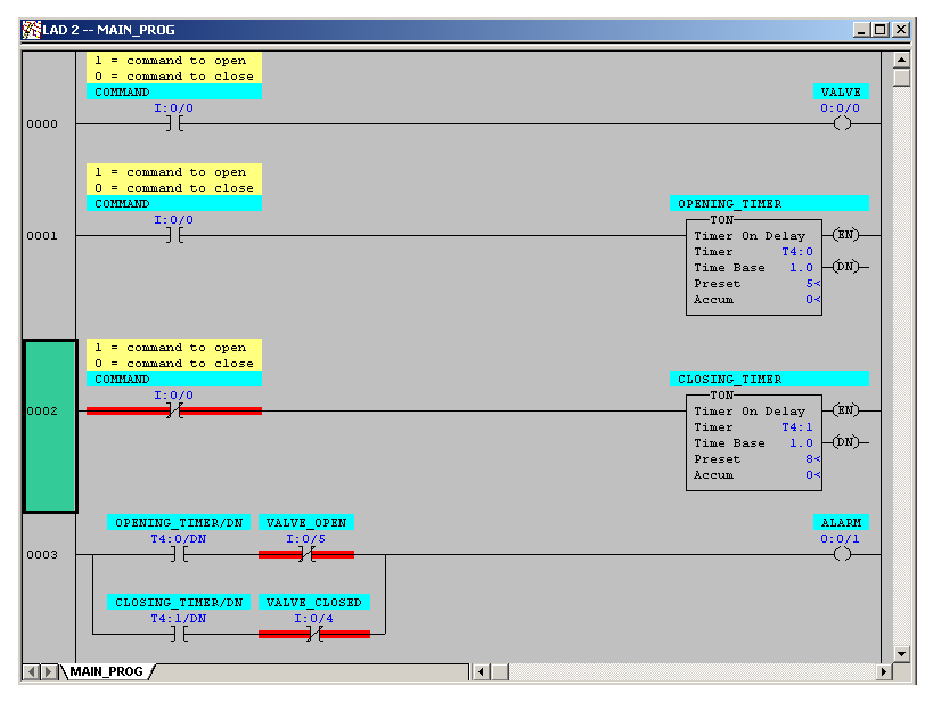
\includegraphics[width=15.5cm]{i02383x01.eps}$$

\vskip 20pt

Based on this program, determine the necessary connections for each limit switch monitoring the valve stem's position:

\begin{itemize}
\item{} {\tt VALVE\_OPEN} limit switch: {\it normally-open} (NO) or {\it normally-closed} (NC)?
\vskip 5pt
\item{} {\tt VALVE\_CLOSED} limit switch: {\it normally-open} (NO) or {\it normally-closed} (NC)?
\end{itemize}

\vskip 20pt

Furthermore, determine the energization status of the PLC output controlling the valve actuator:

\begin{itemize}
\item{} {\tt VALVE} discrete output channel: {\it energize} to open the valve or {\it de-energize} to open the valve?
\end{itemize}

\vfil
\underbar{file i02383}
\eject
%(END_QUESTION)





%(BEGIN_ANSWER)

This is a graded question -- no answers or hints given!

%(END_ANSWER)





%(BEGIN_NOTES)

The limit switch contact instructions in the alarm output rung are both normally-closed.  This means they will be colored -- and therefore have the potential to activate the alarm bit -- when they are in their resting state: when the real-world PLC input channels are de-energized.  This means a de-energized state for both limit switch inputs must correspond to the valve being in mid-position, neither fully open nor fully closed.  Thus, each limit switch must {\it close} when it reaches its travel limit.  A limit switch that closes when actuated, and is open while at rest, is a {\it normally-open} (NO) limit switch.  Thus, both the real-world {\tt VALVE\_OPEN} and {\tt VALVE\_CLOSED} limit switches must be wired with normally-open (NO) electrical contacts.

\vskip 10pt

We can see that the valve control bit is programmed to be the same state as the command input signal {\tt I:0.0}, which also directly activates the ``Opening'' timer instruction.  The ``Closing'' timer instruction is activated whenever {\tt I:0/0} is zero, which will be when the valve control output ({\tt O:0/0}) is zero as well.  Thus, we may conclude that the discrete output {\tt O:0/0} controlling the valve motion will be energized to open the valve, and de-energized to close the valve.


%INDEX% PLC, ladder logic programming: determining necessary switch types from program

%(END_NOTES)


